\documentclass{article}
\usepackage[UTF8, heading = false, scheme = plain]{ctex}

\usepackage{geometry}
\geometry{b5paper,left=2cm,right=2cm,top=2cm,bottom=2cm}

\usepackage{color}
\usepackage{amsfonts}
\usepackage{amsmath}

\linespread{1.5}

\usepackage[colorlinks,
            linkcolor=red,
            anchorcolor=blue,
            citecolor=green
            ]{hyperref}

\usepackage{listings}
\usepackage{fontspec}
\usepackage{graphicx}
\usepackage{algorithmic}
\newfontfamily\monaco{Monaco}
\definecolor{dkgreen}{rgb}{0,0.6,0}
\definecolor{gray}{rgb}{0.5,0.5,0.5}
\definecolor{mauve}{rgb}{0.58,0,0.82}
\lstset{ %
  basicstyle=\footnotesize\monaco,       % the size of the fonts that are used for the code
  numbers=left,                   % where to put the line-numbers
  numberstyle=\footnotesize\monaco\color{gray},  % the style that is used for the line-numbers
  numbersep=5pt
  stepnumber=1,                   % the step between two line-numbers. If it's 1, each line
                                  % will be numbered
  numbersep=5pt,                  % how far the line-numbers are from the code
  backgroundcolor=\color{white},      % choose the background color. You must add \usepackage{color}
  showspaces=false,               % show spaces adding particular underscores
  showstringspaces=false,         % underline spaces within strings
  showtabs=false,                 % show tabs within strings adding particular underscores
  frame=lines,                   % adds a frame around the code
  rulecolor=\color{black},        % if not set, the frame-color may be changed on line-breaks within not-black text (e.g. commens (green here))
  tabsize=4,                      % sets default tabsize to 2 spaces
  captionpos=t,                   % sets the caption-position to bottom
  breaklines=true,                % sets automatic line breaking
  breakatwhitespace=false,        % sets if automatic breaks should only happen at whitespace
  title=\lstname,                   % show the filename of files included with \lstinputlisting;
                                  % also try caption instead of title
  keywordstyle=\color{blue},          % keyword style
  commentstyle=\color{dkgreen},       % comment style
  stringstyle=\color{mauve},         % string literal style
  escapeinside={\%*}{*)},            % if you want to add LaTeX within your code
  morekeywords={*,...}               % if you want to add more keywords to the set
}

\usepackage{amssymb} 
\usepackage{amsmath}
\usepackage[ruled,vlined]{algorithm2e}

\setlength{\parindent}{2em}

\renewcommand{\G}{\mathbb{G}}
\newcommand{\Z}{\mathbb{Z}}
\newcommand{\Q}{\mathbb{Q}}
\newcommand{\F}{\mathbb{F}}

\newcommand{\Sbox}{\textsf{Sbox}}
\newcommand{\code}[1]{\lstinline!#1!}

\newcommand{\CKDpriv}{\textsf{CKDpriv}}
\newcommand{\CKDpub}{\textsf{CKDpub}}

%%%%%%%处理下划线:_%%%%%%%%%
\usepackage{underscore}
%%%%%%%处理下划线:_%%%%%%%%%

\setlength{\parindent}{2.1em}

%%%设置页眉和页码格式
\usepackage{fancyhdr}
\newcommand{\makeheadrule}{%
\rule[0.85\baselineskip]{\headwidth}{0.5pt}\vskip-.8\baselineskip}%1.5 0.4->0.5
\makeatletter
\renewcommand{\headrule}{%
{\if@fancyplain\let\headrulewidth\plainheadrulewidth\fi
\makeheadrule}}
\makeatother
\pagestyle{fancy}
\fancyhf{}
\fancyhead[r]{\textit{Crypto In Action}}
\fancyfoot[C]{--{~\thepage~}--}
%%%设置页眉和页码格式结束

\usepackage{color}
\newcommand{\red}{\textcolor{red}}
\newcommand{\blue}{\textcolor{blue}}



\begin{document}

\title{深入理解Ed25519}
\author{longcpp \\ \small{longcpp9@gmail.com}}

\maketitle

ECDSA签名算法(基于secp256k1或者secp256r1曲线)是目前主流的数字签名算法.
然而在具体应用ECDSA签名算法时,稍有不慎就会引发诸多问题\footnote{
longcpp. ECDSA 签名机制在区块链领域中的应⽤. 2019.
\url{https://github.com/longcpp/CryptoInAction/tree/master/ecdsa-blockchain-dangers}},
这包括签名过程中对随机数需求会在随机数选取不当的情况下引发多种安全问题,
也包括签名值$(r,s)$的可锻造性在特殊应用场景下(例如区块链场景)引发的干扰,
还包括公钥压缩时总需要额外的一个字节来表示一个比特的信息造成的存储空间浪费.
随着各种问题的出现,也有了应对措施,例如RFC 6979\footnote{
RFC 6979. 
Deterministic Usage of the Digital Signature Algorithm (DSA) and Elliptic Curve Digital Signature Algorithm (ECDSA).
\url{https://tools.ietf.org/html/rfc6979}}
中将签名过程中随机数的随机选取变更为通过私钥和待签名消息
进行确定性行派生过程能够以避开与随机数选取相关的安全问题;
而通过在应用层约束$s$的取值范围,则可以规避可锻造性的问题;
同样通过在应用层的逻辑约束,例如利用素数域上二次剩余\footnote{
Pieter Wuille. Schnorr Signatures for secp256k1. 2018.
\url{https://github.com/sipa/bips/blob/bip-schnorr/bip-schnorr.mediawiki}}
的性质,也可以将压缩公钥的表示从33个字节压缩为32个字节.
在实现方面,尤其是在椭圆曲线点群的加法运算,由于secp256k1和secp256r1曲线上
椭圆曲线点群加法的不完备性(需要判定多种边界条件)使得签名过程的常量时间实现愈发困难.
通过相应技术手段同样可以达到常量实现时间,但也相应增加了实现的难度与代码复杂度,
同时不可避免的会对执行速度产生影响.
虽然secp256k1和secp256r1在构造曲线和选取参数时纳入了工程实现的考量,
例如secp256k1自带的自同态映射\footnote{
longcpp. 基于 secp256k1 的⾃同态映射加速 ECDSA 验签. 2019.
\url{https://github.com/longcpp/CryptoInAction/tree/master/secp256k1-endomorphism}
}能够加速验签操作以及
secp256r1所采用的蒙哥马利友好的(Montgomery Friendly)\footnote{
Gueron, Shay, and Vlad Krasnov. 
Fast prime field elliptic-curve cryptography with 256-bit primes. 
Journal of Cryptographic Engineering 5, no. 2 (2015): 141-151.
\url{https://eprint.iacr.org/2013/816.pdf}}
底层素数域的特征$p$.
但是一个很自然的问题是,数字签名算法的运行效率可否做到更快?借助工程手段以及SIMD指令集的应用,
可以逐步提升执行效率.然而更好安全性与更高的执行效率的诉求,或许无法通过这种小步迭代和缝缝补补方式得到满足.

同时解决前述的应用安全,实现安全以及执行效率的问题,
要求在工程手段之外更为深度的改进,一个自然的方向是重新构建椭圆曲线以及签名机制
以便在多个层次上同时改进:改进底层算术运算加速中层点群运算,中层点群运算适配上层协议,
并同时考虑ECDSA签名机制的问题与局限性加以避免.
EdDSA (Edwards-curve Digital Signature Algorithm)签名机制是这个研究方向上的成果.
EdDSA签名机制是Bernstein等人\footnote{
Bernstein, Daniel J., Niels Duif, Tanja Lange, Peter Schwabe, and Bo-Yin Yang. 
High-speed high-security signatures. Journal of Cryptographic Engineering 2, no. 2 (2012): 77-89.
\url{https://ed25519.cr.yp.to/ed25519-20110926.pdf}}
在2012年设计的基于爱德华曲线(Edwards Curves)的数字签名算法.
%更具体来说是基于扭曲爱德华曲线(Twisted Edwards Curves)的数字签名算法.
EdDSA签名机制是Schnorr签名机制的一个变种,其设计初衷是在不牺牲安全性的前提下提升签名/验签速度,
并同时解决前述的ECDSA在应用方面存在的一些问题.

广泛使用的EdDSA签名机制是基于哈希函数SHA-512和椭圆曲线Edwards25519的Ed25519签名机制.
扭曲爱德华曲线Edwards25519双向有理等价于蒙哥马利曲线Curve25519,
提供大约128比特的安全强度(与secp256k1和secp256r1安全强度一致).
Curve25519是Bernstein\footnote{
Bernstein, Daniel J. Curve25519: new Diffie-Hellman speed records.
In International Workshop on Public Key Cryptography, pp. 207-228. Springer, Berlin, Heidelberg, 2006.
\url{https://cr.yp.to/ecdh/curve25519-20060209.pdf}}
在2005年为了提升ECDH密钥交换协议(Elliptic Curve Diffie-Hellman Key Agreement)效率而提出的蒙哥马利曲线,
并同时提供了高速软件实现,相关文献和代码实现参见Curve25519的网站\footnote{
Daniel J. Bernstein. A state-of-the-art Diffie-Hellman function. \url{https://cr.yp.to/ecdh.html}}.
%\red{实现相关的信息 值得注意的是,C hou在SAC 2017上改进了Curve25519的实现效率}
值得注意的是,在2005年的论文中Curve25519实际上用来指代ECDH密钥交换协议,
然而后来多使用Curve25519指代底层的椭圆曲线,造成了讨论时候的困难.
因此Bernstein在邮件中给出了名词约定规范\footnote{
Daniel J. Bernstein. [Cfrg] 25519 naming.
\url{https://mailarchive.ietf.org/arch/msg/cfrg/-9LEdnzVrE5RORux3Oo_oDDRksU}
},用Curve25519指代底层的椭圆曲线,用X25519指代基于Curve25519的ECDH密钥协议,
本文也遵循这种命名规范.

Curve25519是基于素数域$\F_q, \ q = 2^{255}-19$上的蒙哥马利曲线(Montgomery Curve),
曲线方程为$y^2 = x^3 + 486662x^2 + x$.
Curve25519曲线双向有理等价于(Birational Equivalent)扭曲爱德华曲线(Twisted Edwards Curves) Edwards25519:
$x^2 + y^2 = 1 + (121665/121666)x^2y^2$, 而这条扭曲爱德华曲线则同构于(Isomorphic)
爱德华曲线( Edwards Curves) untwisted-Edwards25519: $-x^2+y^2 = 1 - (121665/121666)x^2y^2$.
%前述的Ed25519签名算法精确来说并不是直接构建在Curve25519曲线上的,
%而是基于扭曲爱德华曲线(Twisted Edwards Curves) twisted-Edwards25519.
为什么X25519直接构建在Curve25519之上, 而Ed25519构建在Edwards25519之上,
并且Curve25519和Twisted-Edwards25519是双向有理等价的.
这是因为ECDH协议和EdDSA协议计算过程中重度依赖的点群运算不同,
这是为更好的适配的上层协议而刻意选择的中层的椭圆曲线点的表示的结果.
在继续深入技术原理之前,我们先看下Ed25519和X25519在工业界的应用情况.

2005年就提出的Curve25519以及X25519起初并没有得到广泛的重视和应用,
然而受Dual_EC_DRBG事件\footnote{
Bernstein, D.J., Lange, T. and Niederhagen, R., 2016. Dual EC: A standardized back door. In The New Codebreakers (pp. 256-281). Springer, Berlin, Heidelberg.
\url{https://projectbullrun.org/dual-ec/documents/dual-ec-20150731.pdf}}
的影响,工业界有了很多关于NIST推荐的密码算法标准的质疑.
也因此,设计规则完全透明,没有版权保护并且效率更高的X25519和Ed25519得到重视.
RFC 7748\footnote{
RFC 7748. https://tools.ietf.org/html/rfc7748.
\url{https://tools.ietf.org/html/rfc7748}
}
中描述了椭圆曲线Curve25519和Curve448,以及基于这两条曲线的ECDH协议规范: X25519和X448.
RFC 8032\footnote{
RFC 8032. Edwards-Curve Digital Signature Algorithm (EdDSA).
\url{https://tools.ietf.org/html/rfc8032}
}
则给出了EdDSA (Edwards-curve Digital Signature Algorithm)签名机制的规范,并给出了
基于两个椭圆曲线Edwards25519和Edwards448的EdDSA算法的具体实例化: 
Ed25519, Ed25519ph, Ed25519ctx, Ed448, Ed448ph.
更多的RFC规则进一步给出了在特定场景下使用X25519或者Ed25519的规范.
RFC 8031\footnote{
RFC 8031. Curve25519 and Curve448 for the Internet Key Exchange Protocol Version 2 (IKEv2) Key Agreement. 
\url{https://tools.ietf.org/html/rfc8031}
}
中给出了在IKEv2使用Curve25519和Curve448进行临时密钥交换的规范.
RFC 8080\footnote{
RFC 8080. Edwards-Curve Digital Security Algorithm (EdDSA) for DNSSEC. 
\url{https://tools.ietf.org/html/rfc8080}
}
中给出了在DNSSEC中使用Ed25519和Ed448的规范.
RFC 8410\footnote{
RFC 8410. Algorithm Identifiers for Ed25519, Ed448, X25519, and X448 for Use in the Internet X.509 Public Key Infrastructure.
\url{https://tools.ietf.org/html/rfc8410}
}
中为算法Ed25519, Ed448, X25519, X448定义了用于PKI体系的X.509证书的标识符.
RFC 8420\footnote{
RFC 8420. Using the Edwards-Curve Digital Signature Algorithm (EdDSA) in the Internet Key Exchange Protocol Version 2 (IKEv2).
\url{https://tools.ietf.org/html/rfc8420}
}
中给出了在IKEv2中使用EdDSA时Ed25519和Ed448的ASN.1 Objects.
RFC 8446\footnote{
RFC 8446. The Transport Layer Security (TLS) Protocol Version 1.3.
\url{https://tools.ietf.org/html/rfc8446}
}
中TLS1.3的算法套件中包含了Ed25519和Ed448.
RFC 8463\footnote{
RFC 8463. A New Cryptographic Signature Method for DomainKeys Identified Mail (DKIM).
\url{https://tools.ietf.org/html/rfc8463}
}
为DomainKeys Identified Mail (DKIM) (RFC 6376)添加了新的签名算法Ed25519-SHA256.

%\section{蒙哥马利曲线与爱德华曲线}

相比secp256k1/secp256r1的Short Weierstrass形式的椭圆曲线表示$y^2 = x^3 + ax + b$,
蒙哥马利曲线$Y^2 = X^3 + AX^2 + X$与爱德华曲线(扭曲爱德华曲线) 
$x^2+y^2 = 1  + dx^2y^2$ ($-X^2+Y^2 = 1  - dX^2Y^2$)较为陌生.
Short Weierstrass, 蒙哥马利曲线以及爱德华曲线都可以通过符号代换与
广义Weierstrass曲线$y^2 + a_1xy + a_3y = x^3 + a_2x^2 + a_4x + a_6$相互转换.
X25519和Ed25519的做依赖的点的运算也都可以转换成为Weierstrass曲线上的点运算,
然而使用特定的曲线形式,对于高效安全的X25519或者Ed25519大有裨益.
以twist-Edwards25519为例,其上的点的加法运算是完备(Complete):
$$
(x_1, y_1) + (x_2, y_2) = \left( \frac{x_1y_2 + y_1x_2}{1 + dx_1x_2y_1y_2}, \frac{y_1y_2 - x_1x_2}{1-dx_1x_2y_1y_2} \right),
$$
并且单位元为点$(0,1)$. 习惯了Short Weierstrass形式下椭圆曲线点加运算的各种边界条件判断,
上面的完备的点加运算,简洁优雅的让人有些意外.更值得注意的是,为了构造椭圆曲线的加法点群,
这里无需引入一个假想的无穷远点来满足群的条件.
接下来我们介绍如何从椭圆曲线的一种形式转换成另一种形式\footnote{
关于曲线变化的介绍主要参考了Bassam El Khoury Seguias的博客
Elliptic Curve Groups – Crypto Theoretical Minimum.
\url{https://delfr.com/prerequisites/elliptic-curve-cryptography/}
},以理解蒙哥马利曲线和扭曲爱德华曲线
形式的采用为X25519密钥交换和Ed25519签名机制带来的益处.

\subsection{从广义Weierstrass约化到Short Weierstrass}

一种构造椭圆曲线的方式是将其定义为满足Weierstrass方程的点的结合
\begin{equation}\label{eq-gw}
E: y^2 + a_1xy + a_3y = x^3 + a_2x^2 + a_4x + a_6,
\end{equation}
如果系数$a_1, a_2, a_3, a_4, a_6$取自域(Field) $\F$, 则$E$就是定义在$\F$上的.
注意所有的有限域都可以写成$\F_p^m$的形式,其中$m$为任意正整数,
而$p$是有限域$\F_p^m$的特征(Characteristic),记为$char(\F_p^m)=p$.
当$p\neq 2$并且$p\neq3$时,可以将广义Weierstrass形式简化成为Short Weierstrass形式,
随着推算的进行,我们会看到排除$p\neq 2$以及$p\neq3$情况的原因.
本文中,默认都是在有限域$\F_p$上的椭圆曲线,别处不再复述.

方程(\ref{eq-gw})等号左边,可以看成关于$y$的一元二次多项式,这意味着总可以找到
$\lambda$满足
$$(y+\lambda)^2 - \lambda^2 = y^2 + a_1xy + a_3y,$$
由于$\lambda$的值与$y$无关,则可以通过符号代换,用$\gamma = y + \lambda$替换$y$
从而将方程(\ref{eq-gw})中的变量$y$消除. 
从上式中可以得到$2y\lambda = a_1xy + a_3y$,也即$\lambda = (a_1x + a_3) / 2$.
由于当$char(\F) = 2$时, $2\equiv 0\mod 2$, 也即在$\F$中2的逆不存在,因此我们要求$char(\F)\neq 2$.
将$\lambda$带入方程(\ref{eq-gw})中得到:
\begin{equation*}
\begin{split}
\gamma^2 & - \frac{a_1x + a_3}{2}^2 =  x^3 + a_2x^2 + a_4x + a_6 \\
\iff \gamma^2 & = \frac{a_1x}{2}^2 + \frac{a_3}{2}^2 + \frac{a_1a_3x}{2} + x^3 + a_2x^2 + a_4x + a_6\\
\iff \gamma^2  & = x^3 + (a_2 + \frac{a_1^2}{4})x^2 + (a_4 + \frac{a_1a_3}{2})x + (a_6 + \frac{a_3^2}{4})
\end{split}
\end{equation*}
继续用$a_2' = a_2 + \frac{a_1^2}{4}, a_4' = a_4 + \frac{a_1a_3}{2}, a_6' = a_6 + \frac{a_3^2}{4}$
进行符号代换,得到:
$$
E: \gamma^2 = x^3 + a_2'x^2 + a_4'x + a_6'
$$
继续化简上述方程的等式右边将$x^2$消除掉即可得到期望的Short Weierstrass形式.
用$\chi = x + \nu$代换$x$,其中$\nu$是按照特意选择的值,在带入上面方程后可以消除掉平方项.
计算过程如下:
\begin{equation*}
\begin{split}
\gamma^2 & = (\chi - \nu)^3 + a_2'(\chi - \nu)^2 + a_4'(\chi - \nu) + a_6' \\
\iff \gamma^2 & = \chi^3 -3\nu\chi^2 + 3\nu^2\chi - \nu^3 + a_2'\chi^2 -2a_2'\nu\chi + a_2'\nu^2 + a_4'\chi - a_4'\nu + a_6' \\
\iff \gamma^2 & = \chi^3 + (a_2' - 3\nu)\chi^2 + (3\nu^2 - 2a_2'\nu + a_4')\chi - \nu^3 + a_2'\nu^2 - a_4'\nu + a_6'\\
\end{split}
\end{equation*}
我们希望消除掉$\chi^2$, 则需要给$\nu$添加约束$a_2'-3\nu = 0$, 意味着需要$\nu = a_2' / 3$.
当$\F$的特征为3的时候, 在$\F$中3没有逆元,因此我们要求$char(\F)\neq3$. 由此我们得到
\begin{equation*}
\begin{split}
\gamma^2 & = \chi^3 + (a_2' - 3\nu)\chi^2 + (3\nu^2 - 2a_2'\nu + a_4')\chi - \nu^3 + a_2'\nu^2 - a_4'\nu + a_6'\\
\iff \gamma^2 & = \chi^3 + \left(a_4'-\frac{(a_2')^2}{3}\right)\chi + \left(a_6' + \frac{2(a_2')^3}{27} - \frac{a_2'a_4'}{3}\right)
\end{split}
\end{equation*}
用符号$x$代换$\chi$, 用$y$代换$\gamma$, 并记
$$a = a_4'-\frac{(a_2')^2}{3},\  b = a_6' + \frac{2(a_2')^3}{27} - \frac{a_2'a_4'}{3}$$
就得到了有限域$\F$上的Short Weierstrass形式
$$E: y^2 = x^3 + ax + b,\ \text{其中}\ a, b \in \F, char(\F) \neq 2 \ \text{且}\ char(\F) \neq 3.$$

接下来考虑在$E:  y^2 = x^3 + ax + b$ (也可记为$E: f(x,y) = y^2 - x^3 + ax + b = 0$)上构建椭圆曲线点群所需的条件.
$E$上两个点的加法运算规则依赖过两点的直线与曲线的另一个交点.
当两个点为同一个点时,则是该点的切线与曲线的另一个交点.
由此需要在点群中的每个点都是可微的(Differentiable).也因此我们想要避开包含奇点(Singularity)的曲线.
接下来考察椭圆曲线在何种情况下会包含奇点.
椭圆曲线$f(x,y) = 0$上一个点$(x_P,y_P)$是奇点的充分必要条件为在该点的偏导数为0,也即:
\begin{equation*}
\begin{split}
f(x_P, y_P) = 0 & \iff y_P^2 - x_P^3 - ax_P - b = 0, \\
 f_x(x_P, y_P) = 0 & \iff  -3x_P^2 - a = 0, \\
 f_y(x_P, y_P) = 0 & \iff 2y_P  = 0
\end{split}
\end{equation*}
则有$y_P = 0$, $x_P^3 + ax_P + b = 0$以及$3x_P^2 + a = 0$.
也即点$(x_P,y_P)$是奇点的充分必要条件$x_P^3 + ax_P + b = 0$以及$3x_P^2 + a = 0$.
注意到$x_P$同时满足是$x^3 + ax + b$以及其导数$3x^2 + a$的根,
则$x_P$是$x^3 + ax + b$的二重根,假设另一个根为$\alpha$,则有
\begin{equation*}
\begin{split}
x^3 + ax + b & = (x-x_P)^2(x-\alpha) = (x^2 -2x_Px + x_P^2)(x-\alpha)\\
 & = x^3 - (2x_P + \alpha)x^2 + (x_P^2 + 2x_P\alpha)x - x_P^2\alpha
\end{split}
\end{equation*}
要使等式成立,则有以下条件:
\begin{equation*}
\begin{split}
2x_P + \alpha = 0 & \iff \alpha = -2x_P, \\
a = x_P^2 + 2x_P\alpha & \iff a = x_P^2 + 2x_P(-2x_P) = -3x_P^2\\
b = - x_P^2\alpha & \iff b = -x_P^2(-2x_P) = 2x_P^3
\end{split}
\end{equation*}
由于$a^3 = -27x_P^6$并且$b^2 = 4x_P^6$,合并两个条件就有
$$
a  = -3x_P^2, b = 2x_P^3 \iff  \Delta = 4a^3 + 27b^2 = 0.
$$
则定义在$\F$上的椭圆曲线$E: f(x,y) = y^2 - x^3 - ax - b = 0, a, b \in \F, char(\F)\neq 2, char(\F)\neq 3$
存在奇点的充分必要条件为$\Delta = 4a^3 + 27b^2 = 0$.
然而还存在一种情况,当过一个点的切线斜率的垂直于横坐标时,
则过该点的曲线没有第三个交点,为了处理这种情况,引入了无穷远点$\mathcal{O}$来处理该特殊情况.
$\mathcal{O}$也在点群中扮演了单位元的角色.
由此,定义在有限域$\F_p$上的基于Short Weierstrass形式的椭圆曲线点群可记为$(E_{a,b}^{W}(\F_p), +^W)$:
\begin{equation*}
\begin{split}
E_{a,b}^{W}(\F_p)= \{(x,y)\in \F_p^2\ | & \ y^2 \equiv x^3 + ax + b \mod p, \\
 & a, b \in \F_p, \Delta = 4a^3 + 27b^2 \neq 0, \ p \notin \{2,3\}\} \cup \{\mathcal{O}^W\},
\end{split}
\end{equation*}
而$+^W$表示对应Short Weierstrass形式的椭圆曲线点群上的加法运算.
对于$E_{a,b}^{W}(\F_p)$中的两个点$P=(x_1,y_1), Q = (x_2, y_2)$,则运算$+^W$按照如下规则计算:
\begin{enumerate}
\item $-\mathcal{O}^W = \mathcal{O}^W$, $-P = (x_ 1, -y_1)$, $\mathcal{O}^W +^W P = P$
\item 如果$Q = -P$, 则$P +^W Q=\mathcal{O}^W$
\item 如果$Q\neq -P$, 则$P +^W Q=(x_3,y_3)$, 其中
\begin{equation*}
\left\{
\begin{array}{ll}
x_3 &= \lambda^2 - x_1 - x_2 \\
y_3 & = -y_1 + \lambda(x_1-x_3) \\
\end{array},
\right.
\lambda = 
\left\{
\begin{array}{ll}
\frac{y_2-y_1}{x_2-x_1}, & x_2\neq x_1\\
\frac{3x_1^2+a}{2y_1}, & x_2 =  x_1\\
\end{array}.
\right.
\end{equation*}
\end{enumerate}


\subsection{蒙哥马利曲线Curve25519}

蒙哥马利曲线是Montgomery在1987年为了加速Lenstra的ECM大数分解算法而提出椭圆曲线形式\footnote{
Montgomery, Peter L. Speeding the Pollard and elliptic curve methods of factorization.
Mathematics of computation 48, no. 177 (1987): 243-264. 
\url{https://www.ams.org/journals/mcom/1987-48-177/S0025-5718-1987-0866113-7/S0025--5718-1987-0866113-7.pdf}}.
2017年Costello等人总结了蒙哥马利曲线及其上的算术运算\footnote{
Costello, Craig, and Benjamin Smith. 
Montgomery curves and their arithmetic. 
Journal of Cryptographic Engineering 8, no. 3 (2018): 227-240.
\url{https://arxiv.org/pdf/1703.01863.pdf}}.
定义在有限域$\F_p, p>2$上的蒙哥马利曲线点群可以表示为$(E_{A,B}^M(\F_p), +^M)$:
\begin{equation*}
\begin{split}
E_{A,B}^M(\F_p) = \{(x,y)\in\F_p^2\  | &\  B y^2 \equiv x^3 + A x^2 + x\mod p, \\
& p >2, A, B \in \F_p, B(A^2-4)\neq 0 \} \cup \{\mathcal{O}^M\},
\end{split}
\end{equation*}
点加运算$+^M$可以通过经典的chord-and-tangent方式推算出来.
蒙哥马利曲线上的点加运算也可以按照经典的割线/切线与曲线的交点的方式定义.
假设蒙哥马利曲线上的点$(x_3, y_3) = (x_1, y_1) +^M (x_2,y_2), P = (x_1, y_1), Q = (x_2, y_2)$, 则有

\begin{equation*}
\left\{
\begin{array}{ll}
x_3 & = B\lambda^2 - (x_1 + x_2) - A\\
y_3 & = (2x_1 + x_2 + A)\lambda - B\lambda^3 - y_1 = \lambda(x_1 - x_2) - y_1\\
\end{array},
\right.
\end{equation*}
其中,
\begin{equation*}
\lambda = 
\left\{
\begin{array}{ll}
(y_2-y_1) / (x_2-x_1),\ \text{if}\ P\neq Q, P \neq -Q,\\
(3x_1^2 + 2Ax_1 + 1) / (2By_1),\ \text{if}\ P = Q,
\end{array}
\right.
\end{equation*}
如果$P=-Q$, 则$P +^M Q = \mathcal{O}$, 
可以注意到$\lambda$是过点$P$和点$Q$的割线(当$P=Q$为切线)的斜率.

接下来展示蒙哥马利形式椭圆曲线点群$(E_{A,B}^M(\F_p), +^M)$
与Short Weierstrass形式椭圆曲线点群$(E_{a,b}^{W}(\F_p), +^W)$之间的转换.
\begin{equation*}
\begin{split}
E_{a,b}^{W}(\F_p)= \{(x,y)\in \F_p^2\ | & \ y^2 \equiv x^3 + ax + b \mod p, \\
 & a, b \in \F_p, \Delta = 4a^3 + 27b^2 \neq 0, \ p \notin \{2,3\}\} \cup \{\mathcal{O}^W\},
\end{split}
\end{equation*}
从$E_{A,B}^M(\F_p)$到$E_{a,b}^{W}(\F_p)$的映射
必须将每一个点$(u,v)\in E_{A,B}^M(\F_p)$映射到$E_{a,b}^{W}(\F_p)$中的一个点$(x,y)$.
先考虑非无穷远点的情况.
进行符号代换$u = xB - \frac{A}{3}, v = yB$
\begin{equation*}
\begin{split}
B\left(y^2B^2\right) & = \left( xB - \frac{A}{3} \right)^3 + 
A \left( xB - \frac{A}{3} \right)^2 +  \left(xB - \frac{A}{3}\right) \\
\iff 
27 y^2 B^3 & = (3xB - A)^3 + 3A(3xB-A)^2 + 9(3xB - A) \\
\iff 
27 B^3 y^2 & = 27B^3x^3 - 9A^2Bx + 27Bx + 2A^3 - 9A \\
\end{split}
\end{equation*}
Short Weierstrass形式要求$y^2$的系数为1,则等式两边除以$27B^3$,
这也同时要求$B\neq 0\mod p$ (以及$B$在$\F_p$有逆元),则有:
\begin{equation*}
\begin{split}
y^2 & = x^3 - \frac{A^2}{3B^2}x + \frac{1}{B^2}x + \frac{2A^3 - 9A}{27B^3} \\
\iff 
y^2 & = x^3 + \frac{3-A^2}{3B^2} x + \frac{2A^3 - 9A}{27B^3} \\
\end{split}
\end{equation*}
再进行符号代换$a = \frac{3-A^2}{3B^2}$和$b = \frac{2A^3 - 9A}{27B^3}$即可得到Short Weierstrass形式.
注意Short Weierstrass形式要求$\Delta = 4a^3 + 27b^2 \neq 0$,等价于要求
\begin{equation*}
\begin{split}
& 4\left(\frac{3-A^2}{3B^2}\right)^3  + 27\left(  \frac{2A^3 - 9A}{27B^3} \right)^2  \neq 0 \\
\iff 
& 4\left(3-A^2\right)^3 + \left(  2A^3 - 9A \right)^2 \neq 0 \iff  A^2 \neq 4.
\end{split}
\end{equation*}
在上述推算过程中,有两个约束$B\neq 0\mod p$以及$A^2\neq 4\mod p$,
可以通过乘法运算合并成$B(A^2-4)\neq 0  \mod p$,也即蒙哥马利曲线对参数$A,B$的约束.
前述的映射中将每一个蒙哥马利形式椭圆曲线上的点映射到了short-Weierstrass形式椭圆曲线上的点,
但是没有一个点能够映射到$\mathcal{O}^W$.因此需要引入$\mathcal{O}^M$并将其映射到$\mathcal{O}^W$.
因此我们有了如下定义的从$E_{A,B}^M(\F_p)$到$E_{a,b}^{W}(\F_p)$的映射$\phi$:
\begin{equation*}
\begin{array}{cc}
& \phi: E_{A,B}^M(\F_p)   \rightarrow E_{a,b}^{W}(\F_p) \\
& \phi(u,v)   \rightarrow  (x,y) = \left( \frac{3u+A}{3B}, \frac{v}{B} \right),\ \text{if}\  (u,v)\neq \mathcal{O}^M \\
& \phi(\mathcal{O}^M) \rightarrow \mathcal{O}^W
\end{array}
\end{equation*}
同样的,也可以将short-Weierstrass形式可以转换为蒙哥马利形式:
\begin{equation*}
\begin{array}{cc}
&\phi^{-1}: E_{a,b}^{W}(\F_p)   \rightarrow  E_{A,B}^M(\F_p)\\
&\phi^{-1}(x, y)   \rightarrow (u,v) = \left(xB - \frac{A}{3}, yB\right),\ \text{if}\  (x, y)\neq \mathcal{O}^W \\
&\phi^{-1}(\mathcal{O}^W) \rightarrow \mathcal{O}^M
\end{array}
\end{equation*}
另外可以注意到,除了需要对无穷远点进行特殊处理之外, $\phi$和$\phi^{-1}$都是$\F_p$上的有理映射(Rational Map),
Short-Weierstrass形式和蒙哥马利形式之间的这种双射关系称为双向有理等价(Birational Equivalence).
注意虽然蒙哥马利形式曲线的都可以转换成short-Weierstrass形式,但反之不然.
只有满足特定条件的 short-Weierstrass 才能转换成蒙哥马利形式\footnote{
Wikipedia. Montgomery curve.
\url{https://en.wikipedia.org/wiki/Montgomery_curve\#Equivalence_with_Weierstrass_curves}}.

取$A = 486662, B = 1, p = 2^{255}-19$就得到了蒙哥马利曲线Curve25519:
$$
y^2 = x^3 + 486662x^2 + x,\  B(A^2-4)\neq 0 \mod (2^{255}-19).
$$
根据前面的讨论,取$a = \frac{3-A^2}{3B^2}$和$b = \frac{2A^3 - 9A}{27B^3}$
可以得到与之双向有理等价的short-Weierstrass形式的曲线方程:
$$
y^2 = x^3 + ax + b, \Delta = 4a^3 + 27b^2 \neq 0\mod (2^{255}-19),
$$
根据Listing~\ref{lst-curve25519-sw}, 得到$a,b,\Delta$的具体值如下
\begin{equation*}
\begin{array}{rl}
a & = \texttt{0x2aaaaaaaaaaaaaaaaaaaaaaaaaaaaaaaaaaaaaaaaaaaaaaaaaaaaa984914a144} \\
b & = \texttt{0x7b425ed097b425ed097b425ed097b425ed097b425ed097b4260b5e9c7710c864} \\
\Delta &= \texttt{0x7fffffffffffffffffffffffffffffffffffffffffffffffffffffc8db3de3cd}\\
\end{array}
\end{equation*}
并且$\Delta\neq 0\mod (2^{255}-19)$满足约束条件.
与secp256k1和secp256r1的$a,b$取值相比较, 这样的$a,b$的值非常不利于高效的工程实现.

\begin{lstlisting}[language = python, caption = Curve25519曲线的short-Weierstrass形式的曲线参数,label=lst-curve25519-sw]
sage: fp = GF(2^255 - 19)
sage: A = fp(486662)
sage: B = fp(1)
sage: hex(int(B * (A^2 - 4)))
'0x3724c21c20'
sage: a = (3 - A^2) * (3 * B^2)^(-1)
sage: b = (2 * A^3 - 9 * A) * (27 * B^3)^-1
sage: hex(int(a))
'0x2aaaaaaaaaaaaaaaaaaaaaaaaaaaaaaaaaaaaaaaaaaaaaaaaaaaaa984914a144L'
sage: hex(int(b))
'0x7b425ed097b425ed097b425ed097b425ed097b425ed097b4260b5e9c7710c864L'
sage: delta = 4 * a^3 + 27 * b^2
sage: hex(int(delta))
'0x7fffffffffffffffffffffffffffffffffffffffffffffffffffffc8db3de3cdL'
\end{lstlisting}

X25519是定义在蒙哥马利曲线Curve25519上的ECDH密钥交换协议,
其特殊之处是由于蒙哥马利曲线的采用,点群的加法运算可以仅利用点的横坐标构建,
也可以利用蒙哥马利阶梯算法(Montgomery Ladder)算法,更容易完成高效的常量时间实现.
下一篇中再具体介绍X25519密钥交换协议.

\subsection{扭曲爱德华曲线 Edwards25519}

爱德华曲线是Harold M. Edwards在2007年提出的椭圆曲线形式\footnote{
Edwards, Harold. 
A normal form for elliptic curves. 
Bulletin of the American mathematical society 44, no. 3 (2007): 393-422.
\url{https://www.ams.org/journals/bull/2007-44-03/S0273-0979-07-01153-6/S0273-0979-07-01153-6.pdf}},
定义在有限域$\F_p, p>2$上的爱德华曲线$E_{d}^{E'}$方程为:
$$
x^2+y^2 = 1 + dx^2y^2, d \in \F_p, d \notin \{0,1\}
$$
如果$(x_1,y_1), (x_2, y_2)$是爱德华曲线上的两个点,则$E_{d}^{E'}$上的加法运算$+^{E'}$
规则如下:
$$
(x_1, y_1) +^{E'} (x_2, y_2) = \left( \frac{x_1y_2 + y_1x_2}{1 + dx_1x_2y_1y_2}, \frac{y_1y_2 - x_1x_2}{1-dx_1x_2y_1y_2} \right),
$$
其中单位元为$(0,1)$, 点$(x,y)$的逆元$-(x,y) = (-x,y)$.
值得注意的是,构建爱德华曲线上的加法点群无需引入无穷远点.
Weierstrass形式曲线上的加法运算规则与过两个点的直线和椭圆曲线的第三个交点紧密相关,
但是对爱德华曲线来说,构建的规则更为复杂.
另外,\blue{如果$d$是$\F_p$上的二次非剩余,则上述点加运算规则是完备的(Complete)}, 无需像$+^W$一样需要特殊
处理无穷远点,两个点相同,两个互为逆元等情况.

2008年Bernstein等人指出有限域上只有一小部分椭圆曲线能够表示为爱德华曲线,
并进一步提出了更为广义的扭曲爱德华曲线(Twisted Edwards Curves)\footnote{
Bernstein, Daniel J., Peter Birkner, Marc Joye, Tanja Lange, and Christiane Peters. 
Twisted edwards curves. 
In International Conference on Cryptology in Africa, pp. 389-405. Springer, Berlin, Heidelberg, 2008.
\url{https://cr.yp.to/newelliptic/twisted-20080313.pdf}}.
有限域$\F_p,p>2$上的蒙哥马利曲线集合与扭曲爱德华曲线集合相同,
也即这两类曲线之间是双向有理等价的.
有限域$\F_p, p>2$上的扭曲爱德华曲线$E_{a,d}^E$的方程为:
$$
ax^2 + y^2 = 1 + dx^2y^2, a, d \in \F_p, ad(a-d)\neq 0.
$$
扭曲爱德华曲线中的参数$a=1$时即为爱德华曲线.
如果$(x_1,y_1), (x_2, y_2)$是扭曲爱德华曲线上的两个点,
则$E_{a,d}^E$上的加法运算$+^E$规则如下:
$$
(x_1, y_1) +^E (x_2, y_2) = \left( \frac{x_1y_2 + y_1x_2}{1 + dx_1x_2y_1y_2}, \frac{y_1y_2 - ax_1x_2}{1-dx_1x_2y_1y_2} \right),
$$
其中,单位元为$(0,1)$,点$(x,y)$的逆元$-(x,y) = (-x,y)$,与爱德华曲线类似这里无需引入无穷远点.
\blue{如果$a$是$\F_p$上的二次剩余而$d$不是,则上述扭曲爱德华曲线上点的加法运算$+^E$是完备的.}
用$(E_{a,d}^E(\F_p), +^E)$表示基于扭曲爱德华曲线的加法点群,其中
\begin{equation*}
\begin{array}{rl}
E_{a,d}^E(\F_p) = \{(x,y)\in\F_p^2 \ | & ax^2 + y^2 \equiv 1 + dx^2y^2, a, d \in \F_p, ad(a-d)\neq 0\, \\
& a\ \text{为二次剩余}, d\ \text{为二次非剩余} \}
\end{array}
\end{equation*}


接下来我们展示扭曲爱德华曲线与蒙哥马利曲线之间的双向有理等价关系.
首先展示如何通过符号变换与代换将扭曲爱德华曲线映射到蒙哥马利曲线.
我们沿用之前蒙哥马利曲线表示$E_{A,B}^M(\F_p)$,并首先展示如何
将$E_{a,d}^E(\F_p)$上的点$(x,y)$映射到$E_{A,B}^M(\F_p)$上的点$(u,v)$.
首先令$x = u/v, y = (u-1)/(u+1)$并进行符号带换,这种代换会将几个特殊的点
排除在外,这包括$E_{A,B}^M(\F_p)$中的无穷远点$\mathcal{O}^M$,
$v\equiv 0 \mod p$的点,以及$u\equiv -1 \mod p$点.
根据$E_{a,d}^E(\F_p)$的方程, $v\equiv 0 \mod p$意味着:
$$u(u^2 + Au + 1) = Bv^2 = 0 \iff u = 0\ \text{或者}\ u^2 + Au + 1 = 0. $$
为了将尽可能多的点纳入映射当中,要求$u^2 + Au + 1 \equiv 0 \mod p$无解.
这就等价于\blue{要求判别式$A^2-4$是$\F_p$中的二次非剩余}.
在这个约束条件下,由于$v\equiv 0 \mod p$被排除点仅有$(u,v) = (0,0)$.
接下来考虑$u\equiv -1 \mod p$的点,根据蒙哥马利曲线方程$B\neq 0\mod p$的前提条件:
$$Bv^2 = A - 2 \iff v^2 = (A -2)/B,$$
同样为了减少被排除的点的个数,\blue{要求$(A -2)/B$是$\F_p$中的二次非剩余}.
在这个条件下,没有点会因为$u\equiv -1 \mod p$被排除.
在前面的论述中,被排除的仅有$E_{A,B}^M(\F_p)$中的无穷远点$\mathcal{O}^M$和$(0,0)$.
$E_{A,B}^M(\F_p)$中剩下点都有$u\neq 0 \mod p$, 而$x = u/v$意味着
也同时排除了$E_{a,d}^E(\F_p)$中$x = 0$的点,这包括$(0,1)$和$(0,-1)$.

排除$E_{A,B}^M(\F_p)$中的$\mathcal{O}^M$, $(0,0)$和
$E_{a,d}^E(\F_p)$中的$(0,1)$, $(0,-1)$之后, 将上述符号代换带入$E_{a,d}^E(\F_p)$方程:
\begin{equation*}
\begin{array}{rl}
ax^2 + y^2 = 1 + dx^2y^2 & \iff  a\left(\frac{u}{v}\right)^2 + \left(\frac{u-1}{u+1}\right)^2 = 1 + d\left(\frac{u}{v}\right)^2\left(\frac{u-1}{u+1}\right)^2\\
\end{array}
\end{equation*}
由于$v \neq 0 \mod p$并且$u\neq -1 \mod p$,等式两边同时乘以$v^2(u+1)^2$可以得到:
\begin{equation*}
\begin{array}{rl}
au^2(u+1)^2 + v^2(u-1)^2 \equiv v^2(u+1)^2 + du^2(u-1)^2 \mod p\\
\iff  (a-d)u^4 + (2a-2d)u^3 + (a-d)u^2 - 4v^2u \equiv 0 \mod p
\end{array}
\end{equation*}
由于$u\neq 0\mod p$, 方程两侧同时乘以$u^{-1}$,得到
\begin{equation*}
\begin{array}{rl}
4v^2 \equiv (a-d)u^3 + (2a-2d)u^2 + (a-d)u \mod p
\end{array}
\end{equation*}
注意到$E_{A,B}^M(\F_p)$的方程中$x^3$的系数为1, 上式中为了使$u^3$的系数为1,
我们\blue{要求$a-d \neq 0\mod p$},则方程两侧同时乘以$(a-d)^{-1}$,得到
\begin{equation*}
\begin{array}{rl}
\left(\frac{4}{a-d}\right)v^2 \equiv u^3 + \left(\frac{2a+2d}{a-d}\right)u^2 + u \mod p
\end{array}
\end{equation*}
令$B = 4/(a-d), A = (2a+2d)/(a-d)$并用$x$代换$u$, $y$代换$v$即可得到蒙哥马利形式曲线方程.
注意到蒙哥马利形式方程要求$B(A^2-4)\neq 0 \mod p$.
由于$B = 4/(a-d)$,显然有$B\neq0\mod p$.
从而仅需要\blue{
\begin{equation*}
\begin{array}{rl}
A^2-4 \neq 0\mod p & \iff \left(\frac{2a+2d}{a-d}\right)^2 - 4 \neq 0\mod p\\
& \iff (a+d)^2 \neq (a-d)^2 \mod p \\
& \iff \blue{ad \neq 0 \mod p}
\end{array}
\end{equation*}}

至此完成了从$(x,y) \in E_{a,d}^E(\F_p) \textbackslash \{(0,1), (0,-1)\}$
到$(u,v) \in E_{A,B}^M(\F_p) \textbackslash \{\mathcal{O}^M, (0,0)\}$映射:
$$(u,v) = \psi(x,y) = \left( \frac{1+y}{1-y}, \frac{1+y}{x(1-y)} \right).$$
这个过程中引入了几个限制条件: 
要求$(A -2)/B$是$\F_p$中的二次非剩余等价于要求
$$
\left(\frac{2a+2d}{a-d} - 2\right) / \frac{4}{a-d} = d
$$
为$\F_p$上的二次非剩余.
要求$A^2-4$是$\F_p$中的二次非剩余等价于要求
$$
\left(\frac{2a+2d}{a-d}\right)^2 - 4 = \frac{16ad}{(a-d)^2}
$$
为$\F_p$上的二次非剩余.由于16和$(a-d)^2$显然是$\F_p$中的二次剩余,
并且两个二次剩余的乘积仍为二次剩余,而两个二次非剩余的乘积也有可能是二次剩余,
因此为了确保$(16ad)/(a-d)^2$为二次非剩余,要求$a$和$d$中一个为
二次剩余,一个为二次非剩余.由于$d$已经被限定为二次非剩余,则只能要求$a$为二次剩余.
另外的两个约束条件$a\neq d\mod p$和$ad\neq 0\mod p$可以写为$ad(a-d)\neq 0\mod p$.
这与$E_{a,d}^E(\F_p)$中关于参数$a$和$d$的约束一致,
或者说$E_{a,d}^E(\F_p)$关于$a$和$d$的约束保证了我们可以计算映射$\psi$.
最后$E_{a,d}^E(\F_p)$和$E_{A,B}^M(\F_p)$中都恰好有两个元素没被映射$\psi$处理,
为$(0,-1), (0,1)$定义特殊的$\psi$映射到$(0,0), \mathcal{O}^M$
也就完成了从$E_{a,d}^E(\F_p)$到$E_{A,B}^M(\F_p)$的完整映射:
\begin{equation*}
\begin{array}{cc}
& \psi:  E_{a,d}^E(\F_p) \rightarrow E_{A,B}^M(\F_p) \\
& (x,y) \rightarrow (u,v) \equiv \psi(x,y) = \left(\frac{1+y}{1-y}, \frac{1+y}{x(1-y)}\right), (x,y)\notin \{(0,1),(0,-1)\}\\
& (0,-1) \rightarrow \psi(0, -1) = (0,0) \\
& (0, 1) \rightarrow \psi(0,1) = \mathcal{O}^M
\end{array}
\end{equation*}

考察逆映射$(u,v) \in E_{A,B}^M(\F_p) \rightarrow  (x,y) \in E_{a,d}^E(\F_p)$,
下面再次给出$E_{A,B}^M(\F_p),\ E_{a,d}^E(\F_p)$的定义:
\begin{equation*}
\begin{split}
E_{A,B}^M(\F_p) = \{(x,y)\in\F_p^2\  | &\  B y^2 \equiv x^3 + A x^2 + x\mod p, \\
& p >2, A, B \in \F_p, B(A^2-4)\neq 0 \} \cup \{\mathcal{O}^M\},
\end{split}
\end{equation*}
\begin{equation*}
\begin{array}{rl}
E_{a,d}^E(\F_p) = \{(x,y)\in\F_p^2 \ | & ax^2 + y^2 \equiv 1 + dx^2y^2, a, d \in \F_p, ad(a-d)\neq 0,\\
& a\ \text{为二次剩余}, d\ \text{为二次非剩余} \}.
\end{array}
\end{equation*}
根据上述的映射$\psi$,当$x\neq 0 \mod p, y \neq 1 \mod p$时,
用$u = \frac{1+y}{1-y}, v =  \frac{1+y}{x(1-y)}$进行代换得到:
\begin{equation*}
\begin{array}{rl}
B\left(\frac{1+y}{x(1-y)}\right)^2 \equiv \left( \frac{1+y}{1-y}\right)^3 + A \left( \frac{1+y}{1-y}\right)^2 + \left( \frac{1+y}{1-y}\right) \mod p,
\end{array}
\end{equation*}
注意$x \equiv 0 \mod p$, 有$y^2 \equiv 1 \mod p$, 
这同时剔除了$E_{a,d}^E(\F_p)$中的两个点$(0,1), (0,-1)$.
当$y =\pm 1\mod p$时, 有$ax^2 \equiv dx^2 \mod p$, 只要$\blue{a\neq d}$,就不会剔除外的点.
根据$x,y$取值的约束,则有
$$u = \frac{1+y}{1-y} = -1-\frac{2}{y-1}, v =  \frac{1+y}{x(1-y)}, x\neq 0, y\neq\pm1 \implies u \neq 0, u\neq -1, v\neq 0 $$
%则$u\neq0, u\neq -1, v\neq 0$.
%将$y=-1$带入$E_{a,d}^E(\F_p)$的方程可以得到$ax^2 = dx^2$, 由于$a\neq d$, 因此无解.
%另外由于$u$仅与$y$的值相关,则$u\neq -1 \mod p$, 这是因为不可能有$(1+y)/(1-y) = -1 \iff y +1 = y - 1$.
%而关于$x,y$的约束也同时限定了$u,v\neq0\mod p$.
$u=0$时, 由于$B\neq 0\mod p$, 根据曲线方程有
$$Bv^2 = 0\mod p \iff v \equiv 0\mod p,$$
也即对于$u$的约束剔除了$E_{A,B}^M(\F_p)$中的点$(0,0)$. 
$u=-1$时,根据曲线方程有
$$By^2 = A-2 \iff y^2  = \frac{A-2}{B},$$
\blue{要求$(A-2)/B$为二次非剩余},则上述方程无解,也即$u\neq -1$的条件没有剔除额外的点.
$v = 0 \mod p$时,根据曲线方程有
$$u(u^2 + Au + 1) \equiv 0 \mod p \iff u \equiv 0 \mod p\ \text{或}\ u^2 + Au + 1 \equiv 0 \mod p,$$
为了尽可能少的剔除点,\blue{要求$A^2-4$是$\F_p$中的二次非剩余},也即$u^2  + Au + 1$在$\F_p$中没有根,
则上述情形中只能是$u \equiv 0 \mod p$, 则关于$v$的约束条件没有剔除额外的点.
上面代换隐式剔除的另一个点是$E_{A,B}^M(\F_p)$中的无穷远点$\mathcal{O}^M$.
上述方程简化之后得到:
\begin{equation*}
\begin{array}{cc}
& B(1+y)^2(1-y) = x^2(1+y)\left( (1+y)^2 + A(1+y)(1-y) + (1-y)^2  \right) \\
& \iff B-By^2 =  (2-A)x^2y^2 + (2+A)x^2 \\
& \iff (2+A)x^2 + By^2 = B - (2-A)x^2y^2\\
& \iff \frac{2+A}{B}x^2 + y^2 = 1 - \frac{2-A}{B}x^2y^2
\end{array}
\end{equation*}
用$a = (A+2)/B, d = (A-2)/B$进行代换,可以得到扭曲爱德华曲线形式. 
由于$A^2-4\neq0\mod p$, 则有
$$ad = \left(\frac{A+2}{B}\right)\left(\frac{A-2}{B}\right) = \frac{A^2-4}{B^2}\neq 0\mod p.$$
并且
$$a-d = \frac{4}{B} \neq 0 \mod p.$$
因此, $E_{a,d}^E(\F_p)$中的条件$ad(a-d)\neq 0$得到满足.
接下来考察 $E_{a,d}^E(\F_p)$对于$a$为二次剩余和$d$为二次非剩余的约束.
根据之前的讨论,可知两个约束条件$(A-2)/B$为二次非剩余和$A^2-4$是的二次非剩余,
转换成$a,d$的约束记为要求$a$为二次剩余,$d$为二次非剩余,与$ E_{a,d}^E(\F_p)$中的要求一致.
由此,得到了以下映射:
\begin{equation*}
\begin{array}{cc}
& \psi^{-1}: E_{A,B}^M(\F_p) \rightarrow   E_{a,d}^E(\F_p)\\
& (u,v) \rightarrow (x,y) \equiv \psi^{-1}(u, v) = \left( \frac{u}{v}, \frac{u-1}{u+1} \right),\ \text{if}\ (u,v)\neq(0,0)\\
& (0,0) \rightarrow \psi^{-1}(0,0) = (0, -1) \\
& \mathcal{O}^M \rightarrow \psi^{-1}(\mathcal{O}^M) = (0,1)
\end{array}
\end{equation*}
%由于映射$\psi$和$\psi^{-1}$的存在,扭曲爱德华曲线$E_{A,B}^M(\F_p)$
%和蒙哥马利曲线$ E_{a,d}^E(\F_p)$之间双向有理等价特性.

Edwards25519是定义在有限域$\F_p, \ p = 2^{255}-19$上
选用参数$a=-1$, $d = \frac{121665}{121666}$的扭曲爱德华曲线:
$-x^2 + y^2 \equiv 1 - (121665/121666) x^2y^2 \mod p$.
Ed25519签名机制是定义在Edwards25519曲线上的变种Schnorr签名.
RFC 8032中总结到, EdDSA签名机制的优势在于: 在多种计算平台上都能达到较高的性能;
签名过程中不需要唯一的随机数,能够避免随机数引发的安全问题; 
对于侧信道攻击等具有更好的免疫效果; 公钥和签名值都较小(Ed25519公钥为32个字节,签名值为64字节);
计算公式是完备(Complete),无需对不相信的点执行点的验证操作;
EdDSA能抵抗碰撞,底层哈希函数的碰撞不会破坏EdDSA签名机制(PureEdDSA).
下一篇中逐条解释每一项特性.


\section{X25519与Ed25519}

\subsection{X25519}

RFC 7748中给出了两条蒙哥马利形式的椭圆曲线Curve25519和Curve448,
其中Curve448是Mike Hamburg在2015年设计的新曲线,旨在提供224比特的安全性\footnote{
Hamburg, Mike. Ed448-Goldilocks, a new elliptic curve. IACR Cryptology ePrint Archive 2015 (2015): 625.
\url{https://eprint.iacr.org/2015/625.pdf}}.
本文仅关注Curve25519及定义在其上的ECDH密钥交换协议X25519.
Curve25519是定义在有限域$\F_p, p = 2^{255}-19$的蒙哥马利形式椭圆曲线$y^2 = x^3 + 486662x^2 + x$,
Curve25519的余因子为8,而X25519实际上定义在Curve25519上的子群,阶为\\
\centerline{\texttt{0x1000000000000000000000000000000014def9dea2f79cd65812631a5cf5d3ed},}
RFC 7748中一开始给出的X25519依赖的点群的基点$G$为\\
\centerline{(\texttt{0x9, 0x20ae19a1b8a086b4e01edd2c7748d14c923d4d7e6d7c61b229e9c5a27eced3d9}).}\\
然而在随后的RFC 7748的勘误\footnote{
RFC 7748 Errata. \url{https://www.rfc-editor.org/errata/rfc7748}}
中将基点$G$的具体值修正为\\
\centerline{(\texttt{0x9, 0x5f51e65e475f794b1fe122d388b72eb36dc2b28192839e4dd6163a5d81312c14}).}\\
这是因为, X25519所依赖的椭圆曲线点群运算只涉及点的横坐标,所以X25519涉及的运算只关心横坐标.
然而由于Curve25519与Edwards25519双向有理等价,而Ed25519所依赖的点群运算同时需要横纵坐标,
并且已经有广泛使用的基点的值.
RFC 7748中给出的基点的值,会映射到Edwards25519时会映射成Edwards2519曲线基点的负值,
因此有了上述修正,以便在双向有理映射的条件下保持Edwards25519和Curve25519的基点保持一致.

\begin{figure}[h]
\centering
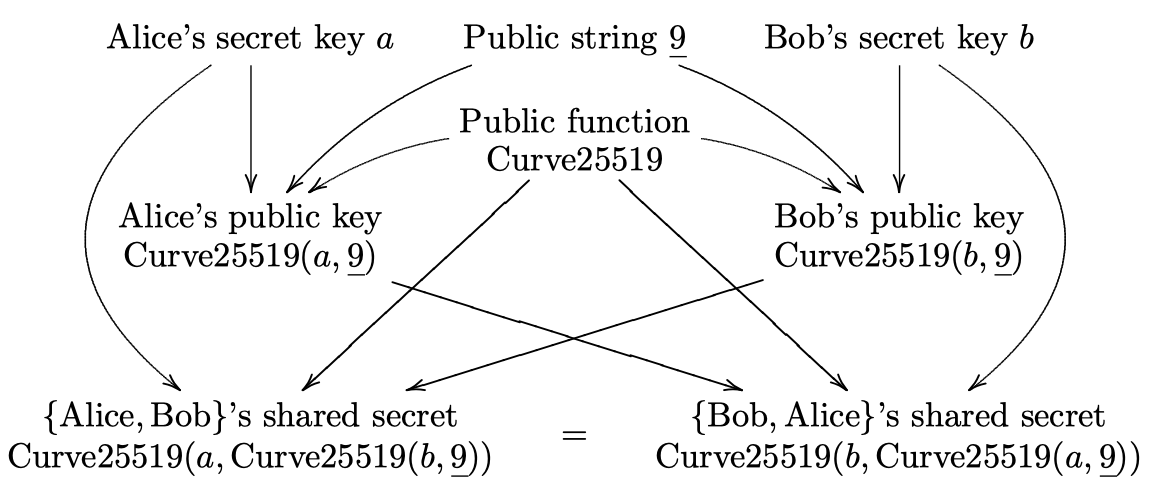
\includegraphics[width=.8\textwidth]{x25519.png}
\caption{X25519密钥交换协议}\label{fig-x25519}
\end{figure}

Alice和Bob之间的ECDH密钥交换协议X25519的执行流程参见Figure~\ref{fig-x25519},
其中'Public string \underline{9}'表示X25519的公共参数基点横坐标的字节数组.
注意这里的点群运算只需要横坐标$x$,用$k$表示标量的话, $x(P)$表示取点$P$的横坐标,
则点的倍乘运算可以表示为$k\cdot x(P)$.
值得提及的是,在X25519和Ed25519的设计文档中,也同时给出了对元素进行编解码的规定.
定义在$\F_p$上的坐标,以小端法编码为字节数组,
也即坐标值$x\in\F_p$与$x[0] + 256  *x[1] + \ldots + 256^{n-1} * x[n-1]$模$p$同余.
从32个字节的数组解码坐标值时,对于X25519协议需要首先将最后一个字节的最高比特位清零,
参见Listing~\ref{lst-x25519-decode}~中第7行,
其中输入参数~\code{bits}~的值为255(对应Curve25519)或者448(对应Curve448).
这个操作的目的是尽可能与基于该曲线的其他协议保持兼容性,因为该比特位通常保留作为标记位.
另外RFC 7748中也明确指出, X25519的协议的实现必须接受非规范(Non-Canonical)的值,
对于X25519而言,非规范的值包括$2^{255}-19$到$2^{255}-1$的所有值.
注意到函数~\code{decodeLittleEndian}~没有对输入参数~\code{u}~做任何限制,
也即32字节的任意值都可以作为Curve25519的公钥$\{\underline{u}, u\in \{0,1,\ldots,2^{256}-1\}\}$.

\begin{lstlisting}[language=python, caption=X25519和X448的编解码, label=lst-x25519-decode]
def decodeLittleEndian(b, bits):
    return sum([ b[i] << 8*i for i in range((bits+7)//8) ])

def decodeUCoordinate(u, bits):
    u_list = [b for b in u]
    # Ignore any unused bits.
    if bits % 8:
        u_list[-1] &= (1 << (bits % 8)) - 1
    return decodeLittleEndian(u_list, bits)

def encodeUCoordinate(u, bits):
    return bytearray([ (u >> 8*i) & 0xff for i in range((bits+7)//8) ])

def decodeScalar25519(k):
    k_list = [b for b in k]
    k_list[0] &= 248  # 1111 1000
    k_list[31] &= 127 # 0111 1111
    k_list[31] |= 64  # 0100 0000
    return decodeLittleEndian(k_list, 255)

def decodeScalar448(k):
    k_list = [b for b in k]
    k_list[0] &= 252
    k_list[55] |= 128
    return decodeLittleEndian(k_list, 448)
\end{lstlisting}

考虑$k\cdot x(P)$中的标量$k$的解析,参见Listing~\ref{lst-x25519-decode}~中的函数~\code{decodeScalar25519}.
与解码坐标值时类似,解码$k$时将32个字节的数组看成是小端法表示的$k$,
但是按照小端法将字节数组转换成标量$k$之前,
需要将最低3比特清零(第16行), 将最高位清零(第17行), 并将紧邻最高位的比特设置为1 (第19行).
也即Curve25519的私钥取值空间为$\{\underline{k}: k\in 2^{254} + 8\cdot\{0,1,\ldots,2^{251}-1\}\}$.
将最低3比特清零可以保证私钥值是8的倍数,考虑到Curve25519曲线的余因子为8,
这样可以避免small-subgroup一类的攻击.
将最高位清零,猜测是为了与公钥的处理方式保持一致.
将紧邻最高位的比特设置为1,有利于常量时间的蒙哥马利阶梯算法实现\footnote{
StackExchange: When using Curve25519, why does the private key always have a fixed bit at 2\^{}254?
\url{https://crypto.stackexchange.com/questions/11810/when-using-curve25519-why-does-the-private-
key-always-have-a-fixed-bit-at-2254/11818\#11818}}.
与secp256k1或者secp256r1等曲线的私钥可以在某个区间内连续取值(整数值)不同,
Curve25519私钥并不是某个区间内的连续取值.
%另外点的倍乘$k\cdot x(P)$可以看做是两个集合到一个集合的映射(非满射):
%$$\{\underline{k}: k\in 2^{254} + 8\cdot\{0,\ldots,2^{251}-1\}\} \times \{\underline{u}, u\in \{0,\ldots,2^{256}-1\}\} \rightarrow \{\underline{u}, u\in \{0,\ldots,2^{256}-1\}\}.$$
%\red{todo: 论证该映射存在的合理性}

前面已经提过到Curve25519上的点群中的加法运算可以仅基于横坐标构建,
第一次见到仅依赖横坐标的点群运算,感觉上非常诡异.
考虑椭圆曲线上点的横坐标与点的关系,可以帮助消除诡异的感觉.
点$P=(x,y)$\textit{基本上}可以仅根据横坐标$x$和曲线方程计算出来,
然而这种计算会得到两个结果$P=(x,y)$以及$-P = (x, -y)$.
由于点和横坐标不是一一对应的,无法通过直接从基于$(x,y)$的点群运算中推导出仅基于横坐标$x$的点群运算.
用$\ominus$表示椭圆曲线$E$上的点的逆映射($\ominus(P) = -P$),定义如下映射$\mathbf{x}$和商群(Quotient Group) $\xi$:
$$\mathbf{x}: E \rightarrow\xi \cong E/\langle\ominus\rangle$$
映射$\mathbf{x}$将$E$中的点送入关于映射$\ominus$的商群$\xi$中:
$$\mathbf{x}(P) = \mathbf{x}(Q) \iff P = Q\ \text{or}\ P = \ominus(Q), P, Q \in E, \mathbf{x}(P), \mathbf{x}(Q) \in \xi.$$
直观上理解, 拥有相同横坐标的点$P, -P$在商群$\xi$中坍缩成同一个元素$\mathbf{x}(P)=\mathbf{x}(-P)$.
并且点$P, -P$的$k$倍乘运算在商群$\xi$中也坍缩成同一个元素.
$$k(-P) = -kP \implies \mathbf{x}(k(-P)) = \mathbf{x}(-kP)= \mathbf{x}(kP).$$
由此, 虽然$\xi$并没有直接从$E$中继承运算,但是签署两个点共享同一个横坐标的问题得到解决,
则$\xi$中可以定义仅依赖于横坐标的运算,并且根据$\xi$和$E$之间的关系,
该运算规则可以根据$E$中的点的加法运算进行推导.
而为了支持高速的ECDH密钥协商,要求能够在$\xi$中根据$\mathbf{x}(P)$和标量$k$快速计算$\mathbf{x}(kP)$.
接下来的问题,就变成了如何构建具有这种形式的椭圆曲线?

蒙哥马利曲线的提出为这一个问题提供了答案,
其中蒙哥马利阶梯(Montgomery Ladder)算法可以根据$\mathbf{x}(P)$和标量$k$快速计算$\mathbf{x}(kP)$,
而蒙哥马利曲线的选择可以保证蒙哥马利阶梯算法中的每一步都可以高效执行.

\begin{figure}[h]
\centering
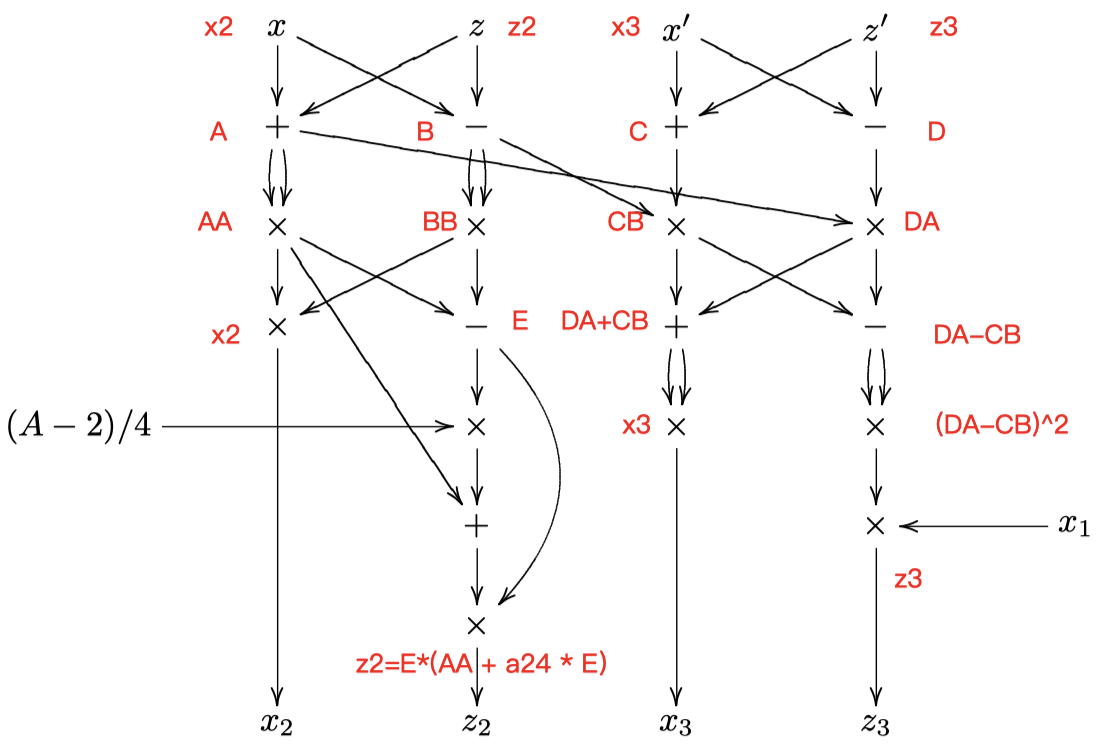
\includegraphics[width=.8\textwidth]{x-coordiniate-add.png}
\caption{X25519密钥交换依赖的点运算}\label{fig-xadd}
\end{figure}

\begin{lstlisting}[language=python, caption = Curve25519和Curve448上的乘法运算, label=lst-curve25519mul]
# Finite field with p
def FiniteField(p):
    class Fp:
        def __init__(self, val: int):
            assert isinstance(val, int)
            self.val = val
        def __add__(self, other):
            return Fp((self.val + other.val) % Fp.p)
        def __sub__(self, other):
            return Fp((self.val - other.val) % Fp.p)
        def __mul__(self, other):
            return Fp((self.val * other.val) % Fp.p)
        def __rmul__(self, n):
            return Fp((self.val * n) % Fp.p)
        def __pow__(self, e):
            return Fp(pow(self.val, e, Fp.p))
        def __repr__(self):
            return hex(self.val)
        def __int__(self):
            return int(self.val)
    Fp.p = p
    return Fp

def cswap(swap, x_2, x_3):
    "Conditional swap in constant time."
    dummy = swap * (x_2 - x_3)
    x_2 = x_2 - dummy
    x_3 = x_3 + dummy
    return x_2, x_3

def mul(k: int, u: int, bits: int, p: int, a24: int):
    Fp = FiniteField(p)
    x_1 = Fp(u)
    x_2 = Fp(1)
    z_2 = Fp(0)
    x_3 = Fp(u)
    z_3 = Fp(1)
    swap = 0

    for t in range(bits-1, -1, -1):
        k_t = (k >> t) & 1
        swap ^= k_t
        (x_2, x_3) = cswap(swap, x_2, x_3)
        (z_2, z_3) = cswap(swap, z_2, z_3)
        swap = k_t

        A = x_2 + z_2
        AA = A**2
        B = x_2 - z_2
        BB = B**2
        E = AA - BB
        C = x_3 + z_3
        D = x_3 - z_3
        DA = D * A
        CB = C * B
        x_3 = (DA + CB)**2
        z_3 = x_1 * (DA - CB)**2
        x_2 = AA * BB
        z_2 = E * (AA + a24 * E)

    x_2, x_3 = cswap(swap, x_2, x_3)
    z_2, z_3 = cswap(swap, z_2, z_3)
    res = x_2 * (z_2**(p - 2))
    return res
\end{lstlisting}

\begin{lstlisting}[language=python, caption = X25519与X448的Python示例, label=lst-x25519x448]
def x25519(k: bytes, u: bytes):
    # Curve25519 for the ~128-bit security level.
    # Computes u := k * u where k is the scalar and u is the u-coordinate.
    bits = 255
    k = decodeScalar25519(k)
    u = decodeUCoordinate(u, bits)
    p = 2**255 - 19
    a24 = 121665
    res = mul(k, u, bits, p, a24)
    return encodeUCoordinate(int(res), bits)

def x448(k: bytes, u: bytes):
    # Curve448 for the ~224-bit security level.
    bits = 448
    k = decodeScalar448(k)
    u = decodeUCoordinate(u, bits)
    p = 2**448 - 2**224 - 1
    a24 = 39081
    res = mul(k, u, bits, p, a24)
    return encodeUCoordinate(int(res), bits)
\end{lstlisting}


Curve25519上的两个不同点的加法运算规则$(x_3, y_3)$

记Curve25519上的两个点$(x_1,y_1), (x_2, y_2)$相加之后得到的点为$(x_3,y_3)$,则

\end{document}

